%!TEX root = ../phd-thesis-lei-ma.tex
%!TeX spellcheck = en-US


\chapter{\label{chap:basics}Neutrino Oscillations in Vacuum}

Neutrinos are special particles since their flavor eigenstates are not the propagation eigenstates, which leads to neutrino flavor conversions while they propagate. To understand the vacuum neutrino oscillations, we use the two-flavor neutrinos scenario as an example\footnote{In most physical problems, two-flavor scenario is a good approximation. The mass splits between the three mass eigenstates are very different so that the oscillation scales differ a lot for the different mass splits. Qualitatively speaking, the two-flavor scenario captures the significant features of the corresponding mass split.}.

Before we work out the math, I can estimate the frequency of the oscillations between flavors. With the natural units system, frequency is of dimension energy, see Appendix~\ref{chap:app-sec:conventions-subsec:units}. We also notice that the energy of the neutrino,
\begin{align}
E_i^{(v)} & = \sqrt{m_i^2 + p_i^2 } \\
& = p_i \sqrt{\frac{m_i^2}{p_i^2} + 1} \\
& \approx p_i + \frac{1}{2} \frac{m_i^2}{p_i},
\label{chap:basics-section:neutrinos-eqn:energy-taylor}
\end{align}
defines the energy scales in this problem. The reason we kept the second order in Taylor expansion is that we are interested in the difference of energies between different mass eigenstates. We assume the neutrinos have almost the same momenta, i.e., $p_1 \approx p_2$. An overall constant energy term of free particles in quantum mechanics provides a global phase to the wave function, which is not of great interest. The only energy scale in our problem should be proportional to the difference of energies between the two mass eigenstates, $\frac{\delta m^2}{2E}$, where $\delta m^2 = m_2^2-m_1^2$. The frequency of flavor oscillations should be of the order
\begin{equation}
    \omega_{\mathrm v} \sim \frac{\delta m^2}{2E}.
    \label{chap:basics-section:neutrinos-eqn:qualitative-method-frequency}
\end{equation}
We'll show that this is indeed the frequency.

To work out the exact solutions, we utilize the Schr\"{o}dinger equation. The wave function in flavor basis is related to wave function in mass basis through a unitary matrix $\mathbf U$,
\begin{equation}
\Psi^{(f)} = \mathbf{U}\Psi^{(v)},
\end{equation}
where $\Psi^{(f)}$ is the wave function in flavor basis and $\Psi^{(v)}$ is the wave function in vacuum mass basis. Upper index ${}^{(v)}$ or ${}^{(f)}$ is used to denote the basis. The rotation matrix is related to the vacuum mixing angle $\theta_{\mathrm v}$ is
\begin{equation}
\mathbf{U} = \begin{pmatrix} \cos\theta_v & \sin \theta_v \\ -\sin \theta_v & \cos \theta_v \end{pmatrix}.
\end{equation}
In vacuum mass basis, the neutrinos have a free propagation Hamiltonian, which is given by
\begin{equation}
\mathbf H^{(v)} = \begin{pmatrix} E_1 & 0 \\
0 & E_2
\end{pmatrix},
\end{equation}
where $E_i$ is defined in Eqn.~\ref{chap:basics-section:neutrinos-eqn:energy-taylor}.
To first order, the Hamiltonian becomes
\begin{align*}
\mathbf H^{(v)} &= \frac{1}{2E} \begin{pmatrix}
m_1^2 & 0 \\
0 & m_2^2
\end{pmatrix} + E \mathbf{I}\\
& =  \frac{1}{4E} \begin{pmatrix}
m_1^2 - m_2^2 & 0 \\
0 & m_2^2 - m_1^2
\end{pmatrix} \\
&\phantom{=}+ \frac{m_2^2 + m_1^2}{4E} \mathbf{I} + E \mathbf{I},
\end{align*}
where the identity matrices only give us an overall phase so we drop them. With the definition that $\delta m^2 = m_2^2 - m_1^2$ The vacuum Hamiltonian in mass basis is simplify
\begin{equation}
\mathbf H^{(v)} =  \frac{\delta m^2}{4E} \begin{pmatrix}
-1 & 0 \\
0 & 1
\end{pmatrix} = -\frac{\delta m^2}{4E} \sigma_3 = -\frac{\omega_{v}}{2}\sigma_3 ,
\end{equation}
which leads to the simple solution for the wave function in mass basis
\begin{equation}
\Psi^{(v)}(t) = \begin{pmatrix}
c_1(0) e^{i \omega_v t/2 } \\
c_2(0) e^{ -i\omega_v t/2 }
\end{pmatrix}.
\end{equation}
% where the initial condition is
% \begin{equation}
% \Psi_v^{(v)}(0) = \begin{pmatrix}
% c_1(0) \\
% c_2(0)
% \end{pmatrix}.
% \end{equation}
In flavor basis, the wave function at anytime is related to wave function in mass basis,
\begin{align}
\Psi^{(f)}(t) &= \mathbf{U}\Psi^{(v)}(t) \\
& = \begin{pmatrix} \cos\theta_v & \sin \theta_v \\ -\sin \theta_v & \cos \theta_v \end{pmatrix} \begin{pmatrix} c_1(0) e^{i\omega_v t/2 } \\
c_2(0) e^{ -i\omega_v t/2 }    \end{pmatrix} .
\end{align}

In many astrophysical neutrino sources such as the solar core, electron neutrinos are most abundant. Thus initial condition is usually assumed to be electron flavor in the calculation which leads to the survival probability of electron flavor
\begin{equation}
P(\nu_e,t) = 1-\sin^2(2\theta_v)\sin^2\left( \frac{\omega_v t}{2} \right).
\end{equation}
Since neutrinos travel with velocity approximately the speed of light, we use $L = t$ where $L$ is the distance traveled. The survival probability is
\begin{equation}
P(\nu_e,L) =  1-\sin^2(2\theta_v)\sin^2\left( \frac{\omega_v}{2} L \right).
\end{equation}
The important parameter is the oscillation length of the neutrino flavor conversion, $1/\omega_v$. This confirms our qualitative method result Eqn.~\ref{chap:basics-section:neutrinos-eqn:qualitative-method-frequency}. This result plotted in Fig.~\ref{chap:basics-section:neutrinos-fig:vacuum-2-flavor-osc} clearly shows the oscillatory behavior. The oscillation length is determined by characteristic energy scale $\omega_v$, while the oscillation amplitude is determined by $\sin^2(2\theta_v)$.

\begin{figure}
    \centering
    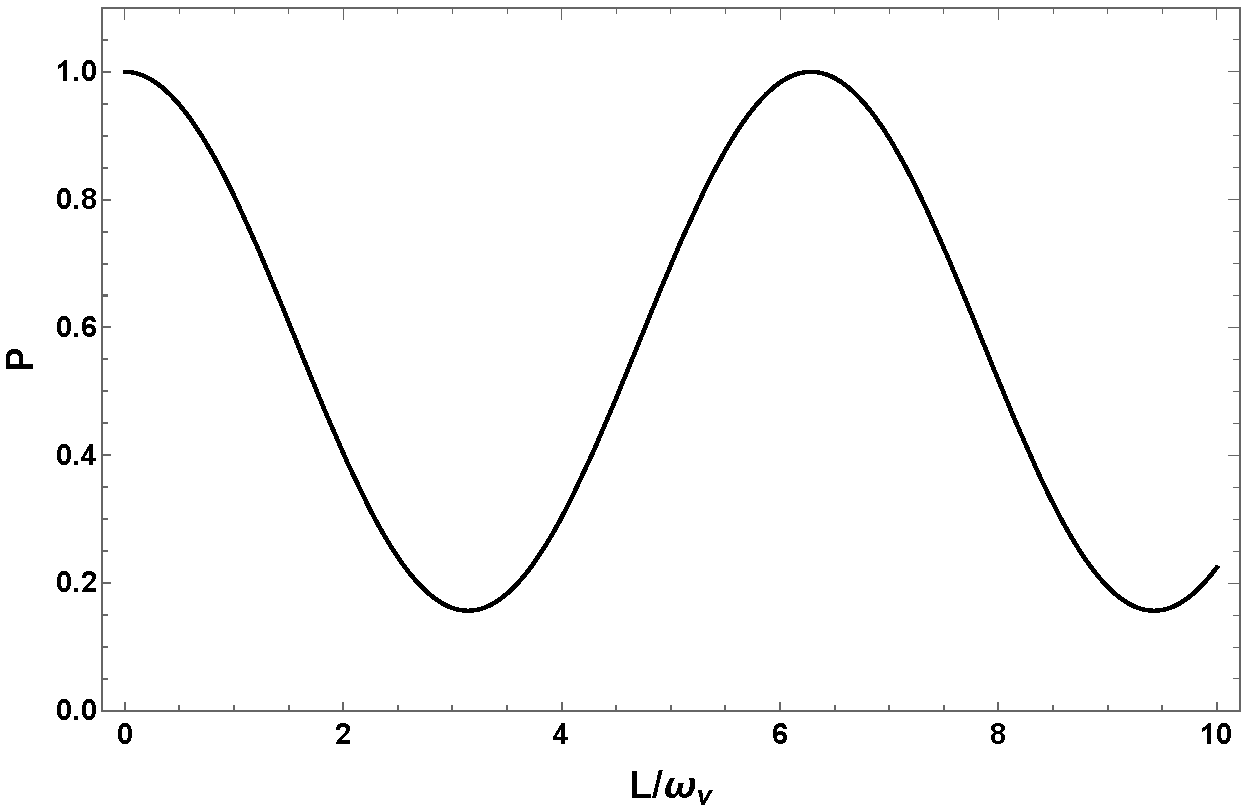
\includegraphics[width=\textwidth]{chapters/assets/basics/neutrino-vaccum-osc-2-flavor.pdf}
    \caption{Electron flavor neutrino survival probability in vacuum oscillations in two flavors scenario. Mixing angle is determined by $\sin^2\theta=0.30 \approx \sin^2 \theta_{12}$.}
    \label{chap:basics-section:neutrinos-fig:vacuum-2-flavor-osc}
\end{figure}

Alternatively, we can find out the Hamiltonian in flavor basis first then solve the Sch\"{o}dinger equation. I will not show the steps here. However, the Hamiltonian in flavor basis is calculated for future use,
\begin{equation}
\mathbf H^{(f)} = -\frac{\omega_v}{2}\cos 2\theta_v \sigma_3 + \frac{\omega_v}{2} \sin 2\theta_v \sigma_1.
    \label{chap:basics-sec:vacuum-osc-eqn:hamiltonian-vacuum}
\end{equation}

\begin{figure}
	\centering
	\begin{subfigure}[t]{0.48\textwidth}
		\centering
		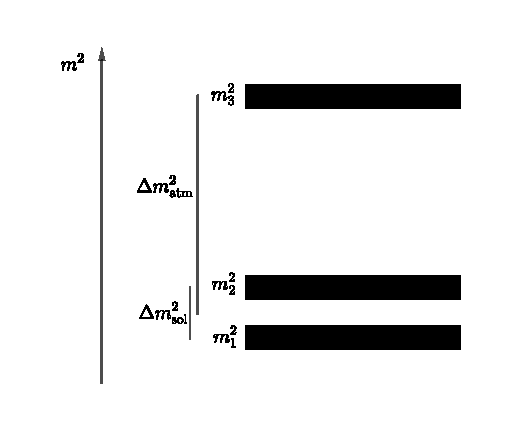
\includegraphics[width=\textwidth]{chapters/assets/basics/masses-nh}
		\caption{Normal hierarchy. The third mass is heavier than the first two masses.}
    \label{chap:basics-sec:flavor-isospin-pic-fig:masses-nh}
	\end{subfigure}
	\quad
	\begin{subfigure}[t]{0.48\textwidth}
		\centering
		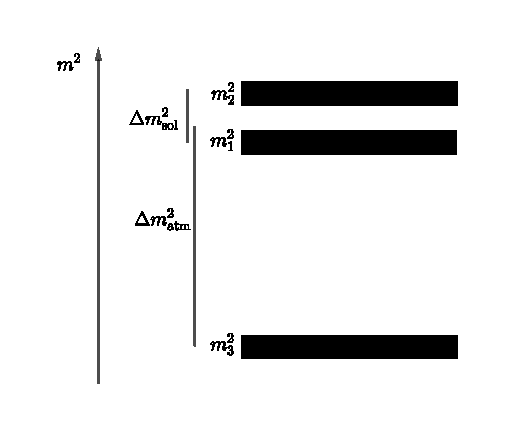
\includegraphics[width=\textwidth]{chapters/assets/basics/masses-ih}
		\caption{Inverted hierarchy. The third mass is smaller than the first two masses.}
    \label{chap:basics-sec:flavor-isospin-pic-fig:masses-ih}
	\end{subfigure}
	\caption{Three masses of neutrinos. The difference between the first two masses is responsible for solar neutrino oscillations and the difference between the third mass and the first two is responsible for atmospheric neutrino oscillations.}
    \label{chap:basics-sec:flavor-isospin-pic-fig:masses}
\end{figure}

\begin{figure}
    \centering
    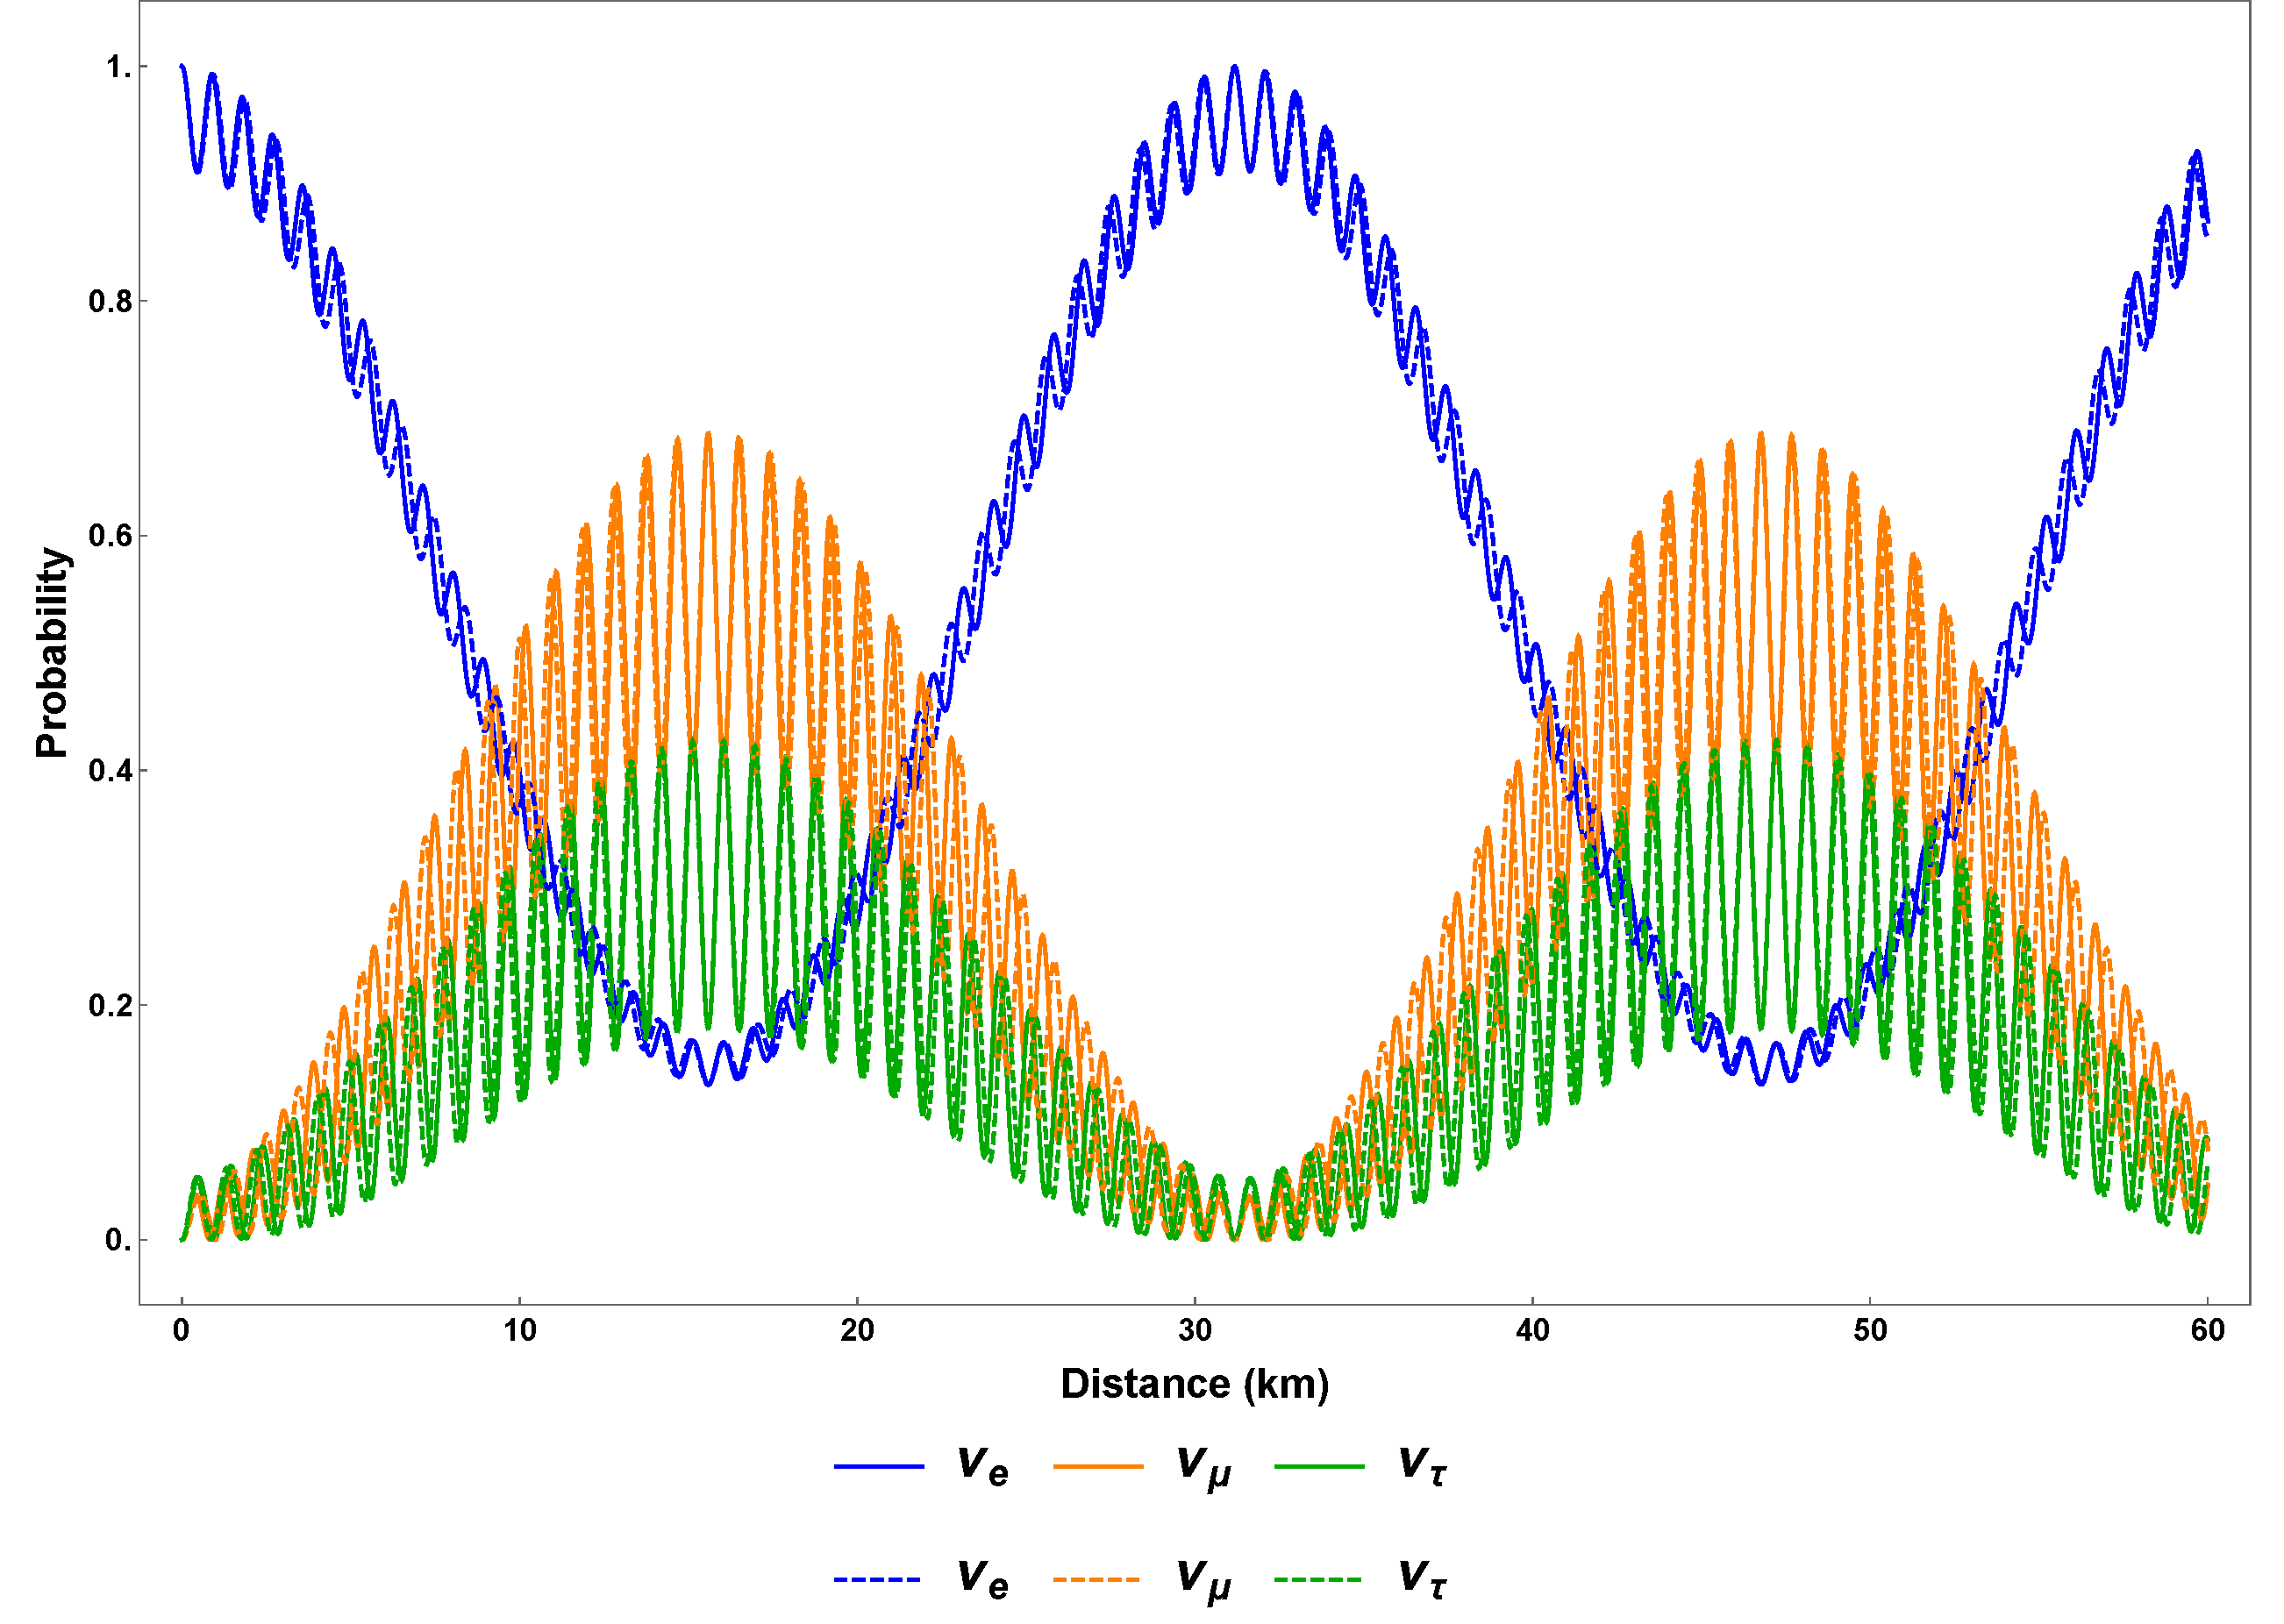
\includegraphics[width=\textwidth]{chapters/assets/basics/vacuum-oscillations-3-flavor.pdf}
    \caption{Neutrino vacuum oscillations with three flavors. The solid lines represent normal hierarchy and the dashed lines represent inverted hierarchy. Mixing angles are determined by $\sin^2\theta_{12}=0.30$, $\sin^2\theta_{13}=0.023$, $\sin^2\theta_{23}=0.41$, while the mass differences are $\delta m_{21}^2 = 7.9\times 10^{-5}\mathrm{eV}$, $\delta m^2_{23}=2.7\times 10^{-3}\mathrm{eV}$. The energy of the neutrinos is 1MeV.}
    \label{chap:basics-section:neutrinos-fig:vacuum-3-flavor-osc}
\end{figure}





In fact, there are three flavors and three masses of neutrinos. The mass squared are shown in Fig.~\ref{chap:basics-sec:flavor-isospin-pic-fig:masses}. We have two quite different characteristic energy scales, $\omega_{v,21}=\delta m_{21}^2/2E$ and $\omega_{v,32}=\delta m_{31}^2/2E$. As for flavor mixing, two oscillation periods should occur, as shown in fig.~\ref{chap:basics-section:neutrinos-fig:vacuum-3-flavor-osc}. The fast oscillations are determined by the larger characteristic energy scale, $\omega_{v,32}$, while the slow oscillations are determined by the smaller one $\omega_{v,21}$. For inverted hierarchy, the oscillation frequencies are the same as normal hierarchy since they have the same characteristic energy scales. However ever they develop different oscillation phases.



\section{\label{chap:basics-sec:flavor-isospin-pic}Flavor Isospin Picture of Neutrino Oscillations}


\begin{figure}
    \centering
    \vspace*{-10pt}
    \includegraphics[width=\textwidth]{chapters/assets/basics/flavor-isospin-illus}
    \caption{In the flavor isospin picture, a flavor isospin pointing upward indicates that the neutrinos are in electron flavor, while the downward direction indicates the other flavor, such as the muon flavor.}
    \label{chap:basics-sec:flavor-isospin-pic-fig:flavor-isospin-illus}
\end{figure}

In principle, the oscillations in two flavor scenario are consequences of the Hamiltonian in this two-level quantum system. It is known that two-level quantum systems are visualized using the Bloch sphere. In the realm of neutrino physics, flavor isospin was introduced for such visualizations~\cite{Duan2006b}. The Hamiltonian for neutrino oscillations in vacuum (Eqn.~\ref{chap:basics-sec:vacuum-osc-eqn:hamiltonian-vacuum}) and in matter (Eqn.~\ref{chap:basics-sec:msw-eqn:hamiltonian-matter-effect}) can be reformulated into vector forms.

We start with the vector form of Hamiltonian for vacuum oscillations. Mathematically speaking, we will cast every two by two matrix into the quaternian basis,
\begin{equation}
    H^{(f)} = - \frac{\vec{\sigma} }{2}\cdot \vec H.
\end{equation}
Meanwhile, the state of neutrinos is represented by the flavor isospin, which is defined as
\begin{equation}
    \vec s = \Psi^{\dagger} \frac{\vec{\sigma} }{2} \Psi.
\end{equation}
As shown in Fig.~\ref{chap:basics-sec:flavor-isospin-pic-fig:flavor-isospin-illus}, the directions of the flavor isospin tell us the flavor content of the neutrino. We choose the direction of the third axis in flavor isospin space to point upward, so that a flavor isospin pointing upward indicates electron flavor by definition. In the flavor isospin formalism, the electron flavor survival probability is related to the third component of the flavor isospin,
\begin{equation*}
P = \frac{1}{2} + s_3.
\end{equation*}
Correspondingly, the equation of motion becomes precession around the Hamiltonian,
\begin{equation}
\dot{\vec s} = \vec s \times \vec H.
\label{chap:basics-sec:flavor-isospin-pic-eqn:eom-precession}
\end{equation}
The precession corresponds to periodic oscillations between flavors.

\begin{figure}
    \centering
    \vspace*{-20pt}
    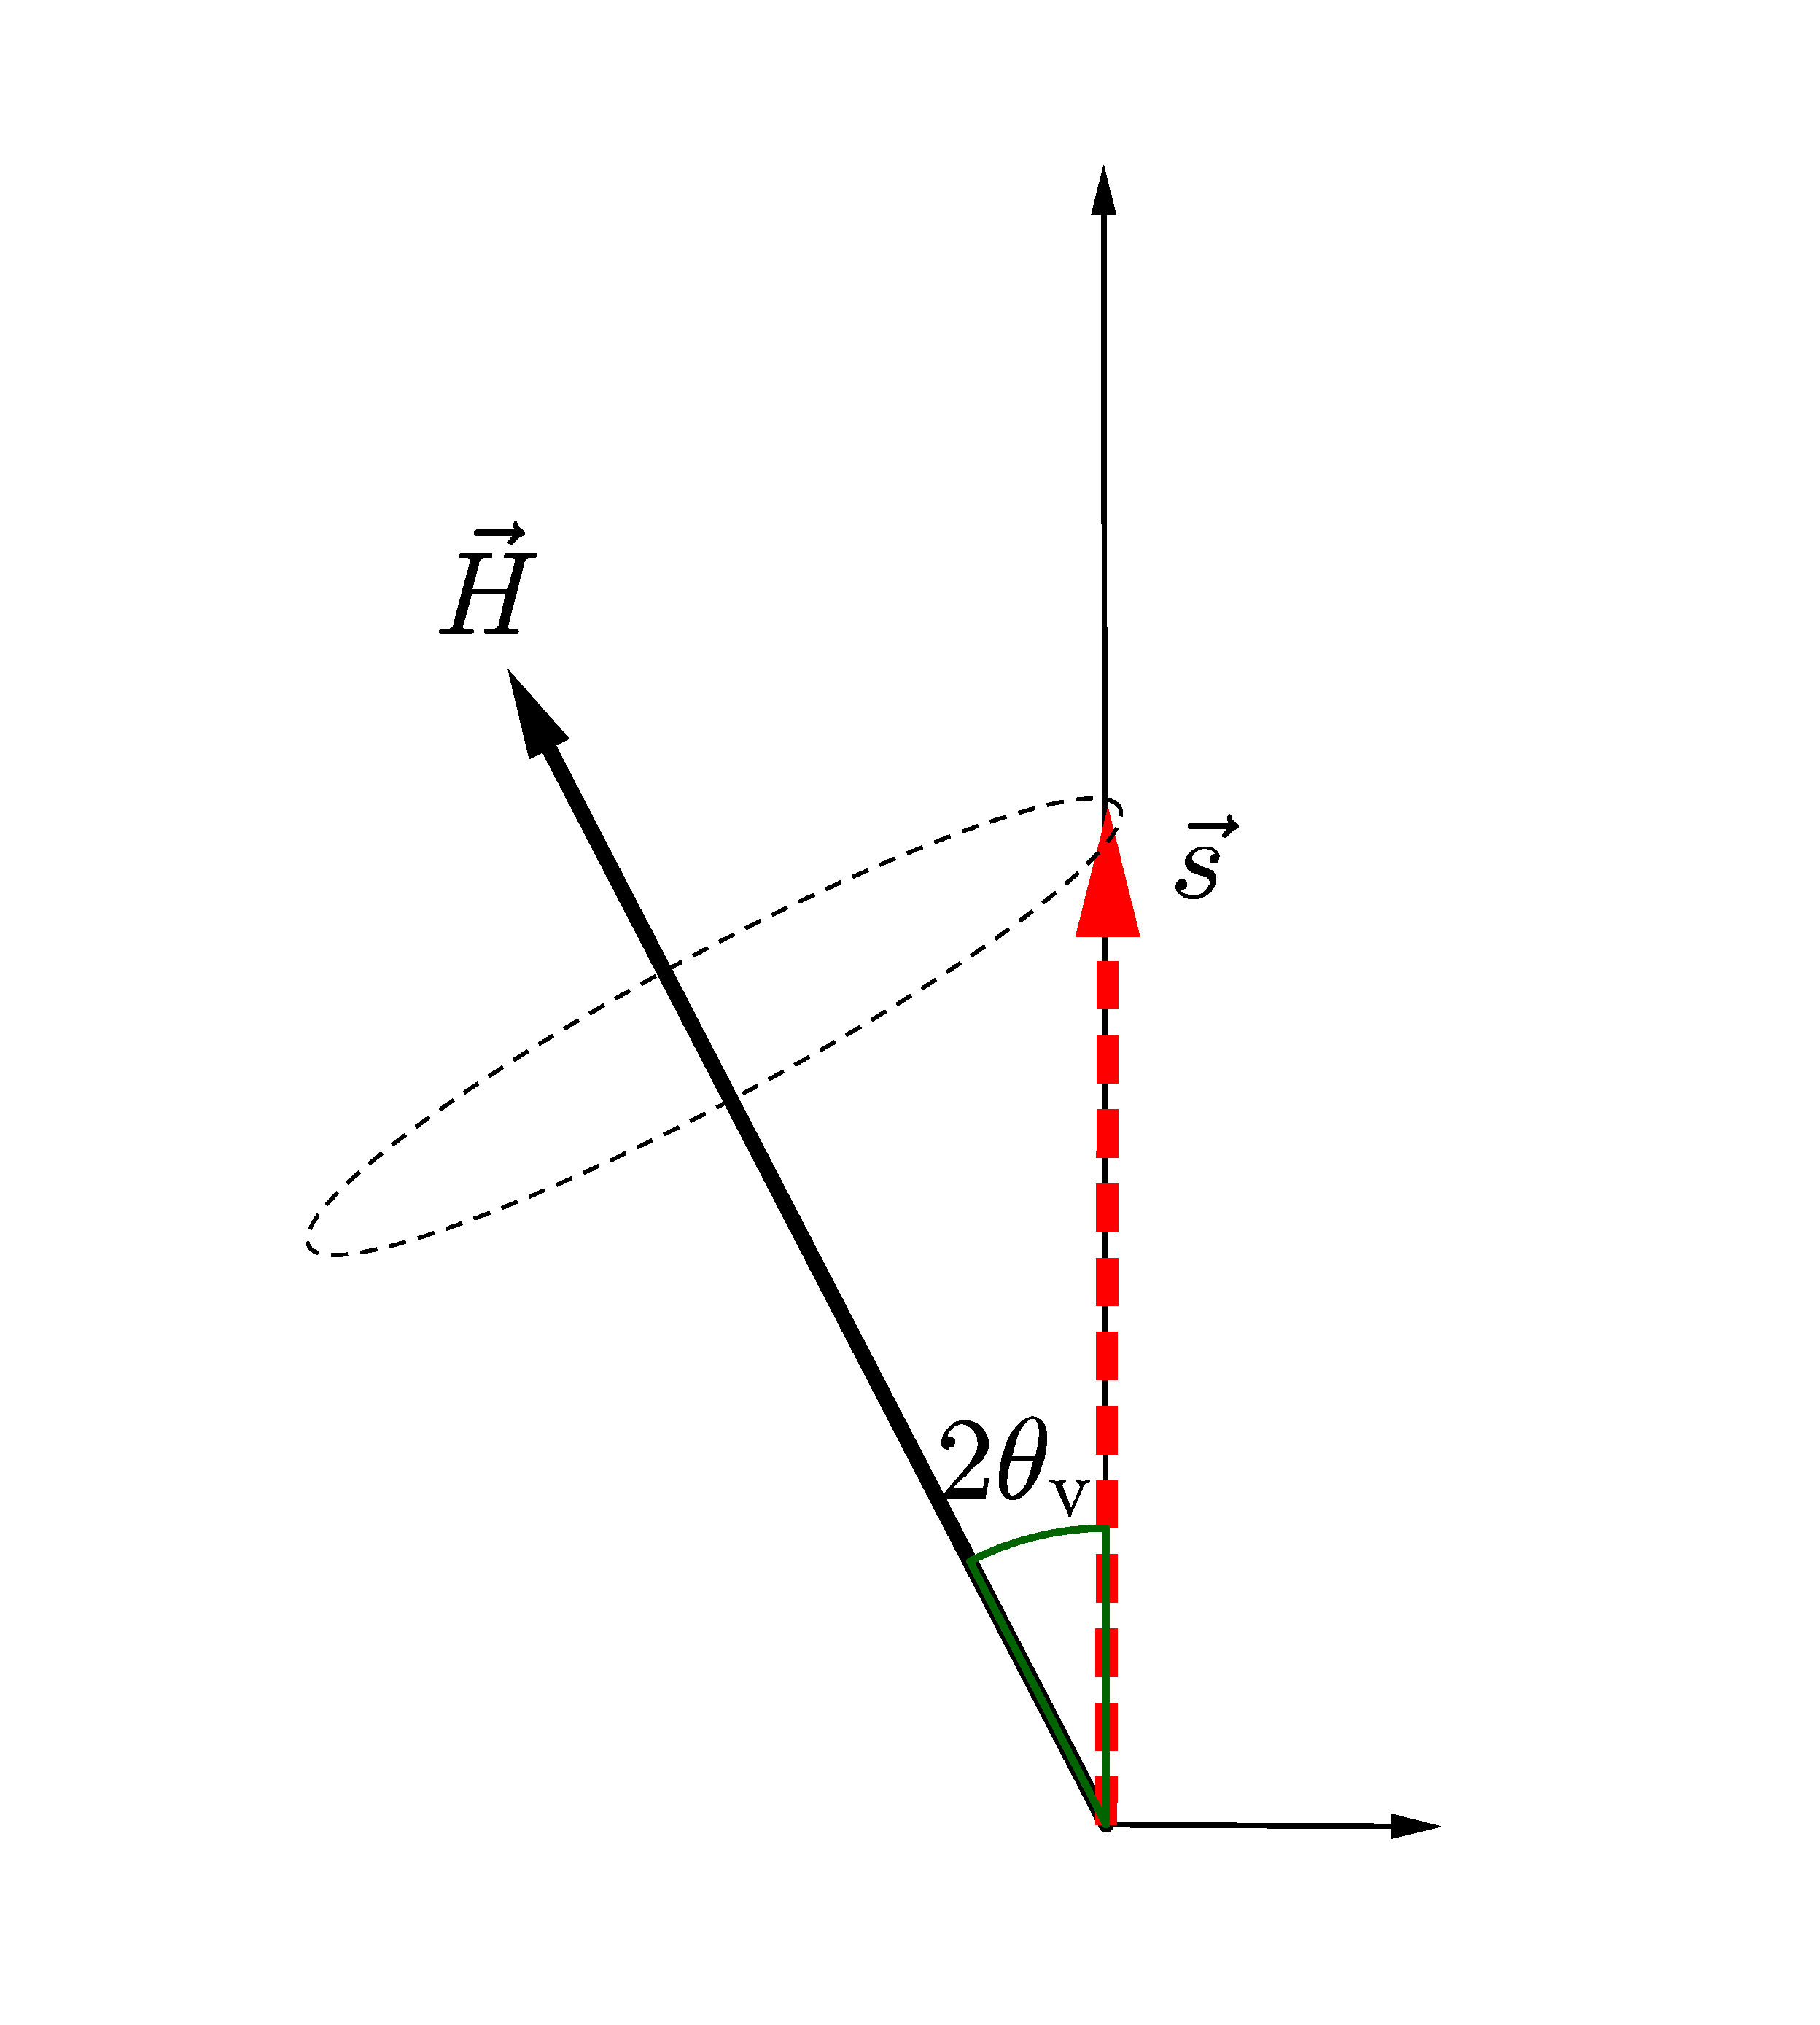
\includegraphics[width=0.7\textwidth]{chapters/assets/basics/flavor-isospin-vac-osc}
    \caption{Vacuum oscillations in flavor isospin picture. Neutrinos starting with electron flavor will follow a precession pattern around the static "Hamiltonian vector" $\vec H$, thus periodic flavor oscillations.}
    \label{chap:basics-sec:flavor-isospin-pic-fig:flavor-isospin-vac-osc}
\end{figure}


For example, in vacuum oscillations, the vacuum oscillation Hamiltonian becomes
\begin{align*}
&\frac{\omega_{\mathrm v} }{2}\left( - \cos 2\theta_{\mathrm v } \sigma_3  + \sin 2\theta_{\mathrm{v}} \sigma_1 \right)
\to  \cos 2\theta_{\mathrm v}\begin{pmatrix}
0\\
0\\
\omega_{\mathrm v}
\end{pmatrix} -\sin 2\theta_{\mathrm v}\begin{pmatrix}
\omega_{\mathrm v}\\
0\\
0
\end{pmatrix},
\end{align*}
which is a vector of length $\omega_{\mathrm v}$ and tilted away from the third axis by the angle $2\theta_{\mathrm v}$. We assume neutrinos start with the electron flavor. Following the equation of motion Eqn.~\ref{chap:basics-sec:flavor-isospin-pic-eqn:eom-precession}, neutrinos precess around vector $\vec H$ that is tilted away from the vertical axis, as shown in Fig.~\ref{chap:basics-sec:flavor-isospin-pic-fig:flavor-isospin-vac-osc}. The oscillation frequency is trivially read out from the precession equation,
\begin{equation*}
    \omega_{\mathrm v} = \lvert \vec H_{\mathrm v} \rvert.
\end{equation*}





\section{Conclusion}

Vacuum neutrino oscillations is easily explained and calculated. However, it conveys the message of the nature of neutrino oscillations. Neutrinos are usually produced in flavor states since they are usually produced in weak interaction. The flavor states do not remain the same during the propagation since the flavor states are not the eigenstates of the propagation Hamiltonian. An extrapolation of this idea is that neutrinos might also oscillate for a constant linear potential. The Hamiltonian would be similar to vacuum Hamiltonian but with different values. One of such situations is neutrinos propagating through a region with constant matter density, which I will explain in next chapter.
